% Generated from MANUSCRIPT_DRAFT.md; regeneration overwrites this TeX file.
\documentclass[lettersize,journal]{IEEEtran}

\usepackage{amsmath,amssymb}
\usepackage{graphicx}
\usepackage{booktabs}
\usepackage{tabularx}
\usepackage{array}
\usepackage{cite}
\usepackage{url}
\usepackage{placeins}
\usepackage[hidelinks]{hyperref}
\graphicspath{{../BEVFusion/riskprop3d_paper/figures/}}
\newcolumntype{Y}{>{\raggedright\arraybackslash}X}
\makeatletter
\setlength{\@fptop}{0pt}
\setlength{\@dblfptop}{0pt}
\setlength{\@fpsep}{12pt}
\setlength{\@dblfpsep}{12pt}
\makeatother
\renewcommand{\dbltopfraction}{0.95}
\renewcommand{\textfraction}{0.05}
\newcommand{\figplaceholder}[1]{%
  \fbox{\parbox[c][32mm][c]{0.94\textwidth}{\centering\bfseries #1}}%
}

\title{Where Does 3D Perception Uncertainty Add Value to Motion Forecasting Under Sensor Degradation?}

\author{Shencheng Zhou, Xinyuan Zhang, and Quan Qian%
\thanks{Shencheng Zhou and Xinyuan Zhang are with the School of Computer Engineering \& Science, Shanghai University, 99 Shangda Road, Baoshan District, Shanghai 200444, China (e-mails: jaycezhou@shu.edu.cn; zhangxinyuan@shu.edu.cn).}%
\thanks{Quan Qian is with the School of Computer Engineering \& Science, Shanghai University; the Center of Materials Informatics and Data Science, Materials Genome Institute, Shanghai University; and the Key Laboratory of Silicate Cultural Relics Conservation (Shanghai University), Ministry of Education, all at 99 Shangda Road, Baoshan District, Shanghai 200444, China.}%
\thanks{Corresponding author: Quan Qian (e-mail: qqian@shu.edu.cn).}}

\begin{document}
\raggedbottom
\maketitle

\begin{abstract}
Motion forecasters inherit uncertainty from three-dimensional perception, but its value depends on how the predictive law enters forecasting. We distinguish stochastic propagation through a fixed host, supervised conditioning on uncertainty representations, and training against a propagated future distribution. A frozen detector fusing camera and laser measurements supplies Gaussian and heavy-tailed/circular laws with shared means. Across six degradation families, the heavy-tailed/circular law consistently improves trajectory energy score in constant-velocity and residual multilayer perceptron probes. On the original final-validation population, the respective reductions are 1.16\% and 1.24\%. A vehicle-only extension integrates current-position uncertainty through a map- and interaction-aware hierarchical vector transformer. The primary energy-score contrast, trained Gaussian minus heavy-tailed/circular, is -0.00063 meters (95\% scene confidence interval, -0.00266 to 0.00135), providing no clear separation. The heavy-tailed/circular law improves over its moment-matched Gaussian surrogate by 0.02311 meters (95\% scene confidence interval, 0.01699 to 0.02984), or 1.40\%. Learned encoders and probability tokens show population- and comparator-dependent benefits. Distribution-preserving training improves teacher fidelity but does not establish a forecasting advantage over an identical ground-truth-only student. The results distinguish complete-law comparisons from moment-matched shape substitutions and show why propagation, representation, and preservation-objective utility require separate evaluation.
\end{abstract}

\begin{IEEEkeywords}
Computer vision; Autonomous driving; Connected and Autonomous Vehicles; motion forecasting; probabilistic 3D perception
\end{IEEEkeywords}

\section{Introduction}
\label{sec:section1}

Motion forecasters infer road-user futures from states reconstructed by perception. Modern architectures represent histories, maps, interactions, and multimodal futures \cite{ref1,ref2,ref3,ref4}, but deployed inputs remain estimates whose quality varies with illumination, point density, calibration, synchronization, and occlusion. Camera--LiDAR fusion improves nominal perception \cite{ref5}, while common-corruption studies show persistent sensitivity to sensor disturbances \cite{ref6,ref7}. Evaluation on curated ground-truth tracks can obscure uncertainty at this perception-to-forecast boundary.

Probabilistic detectors represent current object states as distributions \cite{ref8,ref9}. Forecasting can use these distributions through state samples, learned features, or propagated training targets. Existing work incorporates object-state and map uncertainty through several such interfaces \cite{ref10,ref11,ref12,ref13,ref14,ref15,ref16,ref17}. In joint systems, shared features and queries also carry appearance, context, confidence, and capacity \cite{ref18,ref19,ref20,ref21,ref22}. A benefit at one interface therefore does not establish a benefit at another.

We compare three uses of a common upstream law: stochastic propagation through fixed hosts, supervised conditioning on structured encodings or probability tokens, and distribution-preserving training of an identical student. The original study uses constant-velocity (CV) and residual multilayer perceptron (MLP) probes across six Camera--LiDAR degradation families. A subsequent hierarchical vector transformer (HiVT) extension adds a host that consumes maps and neighboring histories and produces multimodal futures \cite{ref23}. All comparisons concern retained targets with correct identity, allowing state uncertainty to be studied separately from tracking errors.

The paper makes three contributions:

\begin{enumerate}
  \item \textbf{An interface-specific evaluation framework.} Matched controls separate propagation, representation, and preservation-objective utility.
  \item \textbf{Evidence across forecasting configurations.} Six-family CV/MLP experiments and a vehicle-only HiVT extension compare complete trained laws and moment-matched substitutions.
  \item \textbf{A boundary on transferring uncertainty gains.} The trained-law contrast is consistent in simple probes but unresolved in HiVT, whereas the moment-matched contrast remains positive; learned-interface benefits depend on the comparator and population.
\end{enumerate}

\section{Related Work}
\label{sec:section2}

\subsection{Probabilistic 3D perception}
\label{subsec:section2-1}

Uncertainty quantification for autonomous vehicles balances reliability, robustness, accuracy, scalability, and efficiency \cite{ref24}. Camera--LiDAR fusion combines semantic and geometric evidence \cite{ref5}, yet remains sensitive to common corruptions \cite{ref6,ref7}. Probabilistic detectors make localization uncertainty explicit \cite{ref8,ref9}. We compare Gaussian/wrapped-Gaussian and Student-t/von Mises laws that share the decoded state mean, then evaluate the future distributions induced by each law.

\subsection{Forecasting from imperfect perception}
\label{subsec:section2-2}

Map- and interaction-aware predictors model rich context and multimodal behavior \cite{ref1,ref2,ref3,ref4}, \cite{ref23}. Deployment-oriented studies incorporate perceptual uncertainty into forecasting objectives or encoders \cite{ref11,ref12}, quantify sensitivity to noisy object states \cite{ref16}, or model association uncertainty \cite{ref25,ref26}. Joint systems connect perception and prediction through shared features, tracks, and queries \cite{ref18,ref19,ref20,ref21,ref22}, \cite{ref27,ref28}. Our object-centric comparisons condition on correct identity and separate uncertainty information from mean state, confidence, and model capacity.

\subsection{Uncertainty interfaces and distribution preservation}
\label{subsec:section2-3}

Online-map studies propagate positional and semantic uncertainty, characterize favorable scenarios, and use selective gating \cite{ref10}, \cite{ref13,ref14,ref15}. Quantified HD-map uncertainty has also improved HiVT and DenseTNT forecasting \cite{ref17}. These studies establish the value of their respective uncertainty sources and integration designs. We instead hold the object-state mean fixed and ask how the comparison changes across propagation, learned representation, and training objectives.

Distribution distillation approximates an ensemble or predictive law with a single model \cite{ref29}, while perceptual uncertainty also informs planning and proxy driving decisions \cite{ref30,ref31}. Approximation fidelity and forecasting utility are separate endpoints here. We use trajectory energy score to evaluate the full forecast law; minimum-of-sample displacement can reward diversity without properly scoring that law \cite{ref32,ref33,ref34}.

\section{Problem Formulation and Interface Taxonomy}
\label{sec:section3}

\subsection{Object-centric perception uncertainty}
\label{subsec:section3-1}

Let \(\mathcal{S}_{\le t}\) denote Camera--LiDAR observations and matched object history. The detector defines a current-state law

\begin{equation}
\label{eq:current-state-law}
p(X_t\mid\mathcal{S}_{\le t}),
\end{equation}

where \(X_t=(S_t,\Theta_t)\) contains linear 3D box/motion coordinates and yaw. Forecasting seeks a law over six future XY centers,

\begin{equation}
\label{eq:future-trajectory-law}
p(Y_{t+1:t+H}\mid\mathcal{S}_{\le t}),\qquad H=6.
\end{equation}

The analysis is conditional on retained, correctly identified targets. Ground-truth identifiers construct histories and labels; the predictive inputs are detector estimates.

\subsection{Three uncertainty interfaces}
\label{subsec:section3-2}

\subsubsection{Level I: stochastic propagation value}
\label{subsubsec:section3-2-1}

Samples from the current-state law enter a fixed forecasting host:

\begin{equation}
\label{eq:stochastic-propagation}
\begin{aligned}
X_t^{(m)}&\sim p(X_t\mid\mathcal{S}_{\le t}), \\[-1pt]
Y^{(m)}&\sim p_f(Y\mid H_t,X_t^{(m)},B_t), \\[-1pt]
&\quad m=1,\ldots,64.
\end{aligned}
\end{equation}

Here, \(H_t\) is the observed target history and \(B_t\) is the fixed class or scene context. CV and MLP use a deterministic forecast plus shared calibrated Gaussian future noise. HiVT supplies its native multimodal future law. Within each host, changing only the current-state law tests stochastic propagation value.

\subsubsection{Level II: representation utility}
\label{subsubsec:section3-2-2}

A supervised predictor receives a fixed-dimensional representation \(r[p(X_t)]\):

\begin{equation}
\label{eq:learned-representation}
q_\theta(Y\mid H_t,\mu_t,r[p(X_t)],C_t).
\end{equation}

Structured encoders and direct tokens are compared with mean-state, capacity, detector-confidence, and Gaussian-uncertainty controls under the same future supervision.

\subsubsection{Level III: preservation-objective utility}
\label{subsubsec:section3-2-3}

Let \(\pi_t=p_{\mathrm{HTC}}(X_t\mid\mathcal{S}_{\le t})\) denote the heavy-tailed/circular (HTC) law. The 64-sample HTC--MLP pushforward defines a teacher for students receiving the same upstream probability token:

\begin{equation}
\label{eq:preservation-objective}
\begin{aligned}
&\widehat p_{\mathrm{MC}}^{\mathrm{HTC}\rightarrow f}(Y\mid H_t,\pi_t,C_t) \\[-1pt]
&\longrightarrow  q_\theta(Y\mid H_t,\pi_t,C_t).
\end{aligned}
\end{equation}

Identical students are trained with or without distribution preservation. Teacher fidelity measures approximation; the GT-only comparison measures the forecasting utility of the added objective.

\begin{figure*}[!t]
\centering
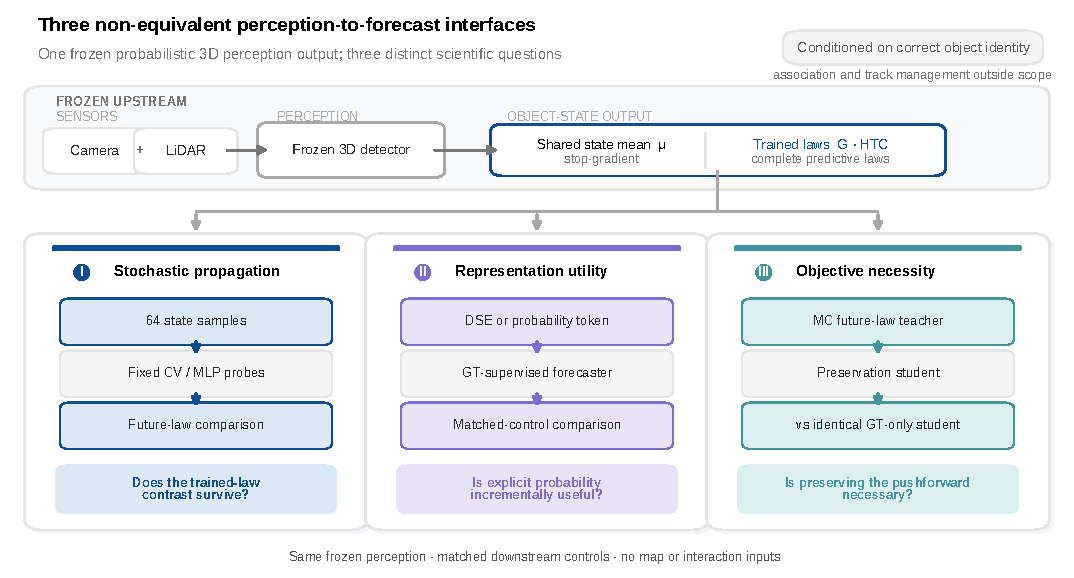
\includegraphics[width=\textwidth]{figure_1_interface_taxonomy.pdf}
\caption{Three perception-to-forecast uncertainty interfaces. Fixed-host propagation compares predictive laws, supervised conditioning compares uncertainty representations, and identical-student training tests preservation-objective utility.}
\label{fig:figure1}
\end{figure*}

\section{Experimental Protocol}
\label{sec:section4}

\subsection{Dataset and target construction}
\label{subsec:section4-1}

The original study uses scene-disjoint nuScenes training, label-calibration, development, and final-validation populations \cite{ref35}. At each frame, 200 TransFusion queries are assigned one-to-one to LiDAR-supported ground-truth objects in the ten detection classes using the native Hungarian cost. Assigned pairs are retained when their BEV centers are within 2.0 m. Histories follow annotation identity through two to four previous keyframes, and labels contain six future centers in the current LiDAR frame. Broken chains and insufficient histories or futures are excluded. Each paired comparison uses identical eligible targets. Section S2 specifies the matching cost, state order, and row construction.

\subsection{Upstream predictive laws}
\label{subsec:section4-2}

The frozen BEVFusion detector uses a Swin-T camera encoder, 0.075-m LiDAR voxels, ConvFuser, and a 200-query TransFusion head \cite{ref5}. Two 18,443-parameter probability heads receive the same query features, class logits, state means, and score while preserving the detector's decoded means. The linear state is \(S_t=[x,y,z,\log w,\log l,\log h,v_x,v_y]\); yaw is modeled separately.

The Gaussian law (\textbf{G}) uses diagonal Gaussian linear coordinates and wrapped-Gaussian yaw:

\begin{equation}
\label{eq:gaussian-perception-law}
\begin{aligned}
p_{\mathrm{G}}(X_t) &=\mathcal N(S_t;\mu_t,\Sigma_t^{\mathrm G}) \\[-1pt]
&\quad {}\,p_{\mathrm{WG}}(\Theta_t;\mu_t^\theta,\sigma_{t,\theta}^2).
\end{aligned}
\end{equation}

The heavy-tailed/circular law (\textbf{HTC}) uses multivariate Student-t linear coordinates and von Mises yaw:

\begin{equation}
\label{eq:htc-perception-law}
\begin{aligned}
p_{\mathrm{HTC}}(X_t) &=t_{\nu_t}(S_t;\mu_t,\Sigma_t^{\mathrm{HTC}}) \\[-1pt]
&\quad {}\,\mathrm{VM}(\Theta_t;\mu_t^\theta,\kappa_t).
\end{aligned}
\end{equation}

Both heads use 20 clean-training epochs on 22,508 samples from 560 scenes, with three paired repetitions. A disjoint 2,814-sample, 70-scene population supplies calibration. G and HTC share means but have independently learned scales, so their comparison concerns complete trained laws. Table 1 characterizes the original heads on clean development. HTC improves linear likelihood and coverage; G has slightly better yaw coverage and smaller equal-coverage static volumes.

A retrospective \textbf{HTC-MMG} control replaces HTC with a Gaussian having the same linear mean and covariance:

\begin{equation}
\label{eq:moment-matched-law}
S_t^{\mathrm{MMG}}\sim\mathcal N\!\left(\mu_t,\frac{\nu_t}{\nu_t-2}\Sigma_t^{\mathrm{HTC}}\right).
\end{equation}

For yaw, the wrapped-Gaussian variance \(-2\log[I_1(\kappa_t)/I_0(\kappa_t)]\) matches the first trigonometric moment. This control tests a higher-order law substitution with the input's low-order moments held fixed.

\begin{table*}[!t]
\caption{Original-head characterization on identical clean-development queries. NLL, coverage, and scales use raw outputs; volume uses empirical 90\% rescaling. Positive NLL contrasts favor HTC.}
\label{tab:table1}
\centering
\footnotesize
\setlength{\tabcolsep}{3pt}
\renewcommand{\arraystretch}{1.15}
\begin{tabularx}{\textwidth}{@{}YY@{}}
\toprule
\textbf{Pre-forecast quantity} & \textbf{Frozen characterization} \\
\midrule
Full-geometry NLL contrast & 4.10243 (95\% CI 1.97022, 7.42856) \\
XY NLL contrast & 0.12799 (0.11494, 0.14169) \\
Yaw NLL contrast & 2.71034 (0.62140, 6.01430) \\
Linear 90\% coverage error (\(\mathrm{coverage}-0.90\)) & G: -0.03827; HTC: +0.01330 \\
Yaw 90\% coverage error (\(\mathrm{coverage}-0.90\)) & G: +0.02549; HTC: +0.03107 \\
Median linear-scale ratio, HTC/G & 0.758--0.791 \\
Equal-coverage 90\% ellipsoid-volume ratio, HTC/G & 1.095--1.249 \\
\bottomrule
\end{tabularx}
\end{table*}

\subsection{Forecasting probes and learned interfaces}
\label{subsec:section4-3}

The original Level-I hosts are map-free CV and a 26,380-parameter residual MLP. Each law uses 64 samples, with common random numbers for compatible G/HTC coordinates. Clean label-calibration residuals fit one zero-mean 2D Gaussian covariance per horizon and host; all laws share these future-noise distributions and draws. A retrospective sensitivity analysis scales the covariances by \(\lambda\in\{0,0.5,1,2\}\).

Learned representation groups share history/class inputs, a six-mode diagonal-Gaussian residual decoder, and GT supervision. Structured controls include mean-only, Gaussianized, no-tail, and no-circular encoders. Direct conditioning uses one 24,118-parameter architecture with mean-only, confidence, G, or HTC tokens. Matched groups share initialization, batches, and epochs. The preservation student adds distribution, moment, calibration--sharpness, and ranking losses to the identical GT-only student. Section S2 specifies architectures and losses.

\subsection{Sensor degradation}
\label{subsec:section4-4}

Development conditions comprise camera lowlight, LiDAR point dropout, and beam reduction at fixed severities. Held-out degradation families comprise camera extrinsic rotation, translation, and temporal offset. Table S2 specifies transformations and retained-target counts. A sensitivity analysis restricts the 15 non-final conditions to 20,580 common targets.

\subsection{Metrics and inference}
\label{subsec:section4-5}

Trajectory energy score (ES) is the primary endpoint \cite{ref32,ref33}. For samples \(Y^{(1)},\ldots,Y^{(M)}\) and target \(y\),

\begin{equation}
\label{eq:trajectory-energy-score}
\begin{aligned} \operatorname{ES} &=\frac{1}{M}\sum_{m=1}^{M}\lVert Y^{(m)}-y\rVert_2 \\ &\quad-\frac{1}{2M(M-1)}\sum_{m\ne n}\lVert Y^{(m)}-Y^{(n)}\rVert_2. \end{aligned}
\end{equation}

Lower ES is better. Diagnostic NLL evaluates the comparison-specific likelihood; mean ADE/FDE assess point accuracy. Original-study sharpness is median final ellipse area rescaled to empirical 90\% coverage. Forecast-error ranking uses final log ellipse area against shared labels from a fixed reference forecast, with failure defined by FDE greater than 2 m (Section S3).

Each comparison averages paired target differences within scene and across three repetitions. Original-study 95\% CIs use 10,000 paired-scene bootstrap resamples and quantify scene variation conditional on these runs; individual directions describe repetition stability. ES is primary, whereas component, ranking, transport, and attribute analyses are secondary or descriptive. Intervals are computed separately without a joint multiplicity claim. Transport associations use a shared-scene bootstrap (Section S3.4).

\subsection{Evaluation chronology}
\label{subsec:section4-6}

The original final-validation population contains 68,436 targets from 6,019 samples in 150 scenes. Its forecasting outcomes were accessed after the original checkpoints, calibration, comparisons, and analysis plan were fixed. Transport, future-noise, and moment-matched analyses followed as retrospective sensitivity studies. The HiVT extension was designed after these outcomes had been observed and reuses the official-validation population; its analysis plan preceded the extension runs. Section S1 records the stages.

\subsection{Map- and interaction-aware HiVT extension}
\label{subsec:section4-7}

The Level-I extension adapts HiVT \cite{ref23} to retained nuScenes vehicles. Three clean-trained hosts consume the target's XY history, neighboring histories re-exported from the same perception condition, and an HD map. Target means, histories, probability-head inputs, identities, and labels retain their original archive values. Three independently restored head pairs supply the extension laws; the original CV/MLP hosts are re-evaluated with these heads on the same vehicles.

Within each HiVT run, the target's current XY law is integrated through its native six-mode Laplace decoder while map and neighbor background remain fixed. A0 uses the mean current position; AG, AH, and AM integrate G, HTC, and HTC-MMG, respectively. A clean-calibrated output-scale multiplier is shared by all four laws. The sole primary contrast is AG-minus-AH on official clean validation. Development clean, dropout S3, rotation S3, and AM-minus-AH are explanatory comparisons. Scene CIs are conditional on the three paired runs. Reported coverage and area use moment ellipses that include between-mode, between-state, and conditional Laplace variance (Section S7).

\section{Results}
\label{sec:section5}

\subsection{HTC improved stochastic propagation in CV and MLP}
\label{subsec:section5-1}

On clean development, HTC reduced ES relative to G by 0.01614 m (95\% CI 0.01102, 0.02150) with CV and 0.01230 m (0.00850, 0.01619) with MLP. Every repetition favored HTC, which also outperformed mean-state propagation. Gains remained positive across the six degradation families. Final-validation reductions were 0.02060 m (0.01632, 0.02532) and 0.02101 m (0.01603, 0.02688), or 1.16\% and 1.24\% (Table 3).

The original development conditions had HTC/G equal-coverage area ratios of 0.866--0.929; final-validation ratios were 0.8549 and 0.8537. The largest HTC-versus-mean ADE/FDE increases were 0.01125/0.01692 m. Future-noise scaling preserved the HTC-over-G direction: increasing \(\lambda\) from 0 to 2 reduced the clean gains from 0.03050 to 0.01108 m for CV and from 0.02290 to 0.00782 m for MLP (Supplementary Fig. S2).

HTC also outperformed HTC-MMG. Clean gains were 0.01663 m (0.01301, 0.02067) and 0.01695 m (0.01325, 0.02112); final-validation gains were 0.01760 m (0.01437, 0.02095) and 0.01763 m (0.01441, 0.02097). This direction held across all six degradation families, with mean ADE/FDE differences below 0.0015 m and a supporting 256-sample analysis (Table S6).

\begin{figure*}[!t]
\centering
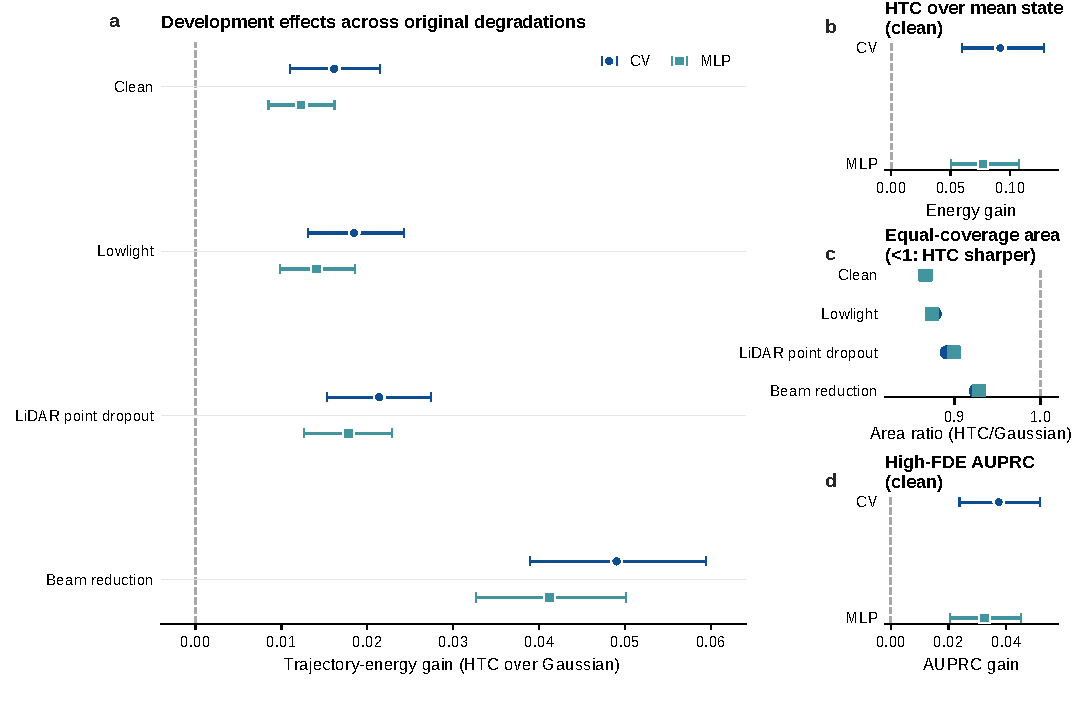
\includegraphics[width=\textwidth]{figure_2_stochastic_propagation.pdf}
\caption{Original development stochastic-propagation results. Circles and squares denote CV and MLP; points average three repetitions and bars give paired scene-bootstrap 95\% CIs. Panels show (a) G-minus-HTC ES, (b) mean-state-minus-HTC ES, (c) HTC/G equal-coverage area ratios, and (d) HTC-minus-G high-FDE AUPRC. Positive differences favor HTC; area ratios below one indicate sharper HTC regions.}
\label{fig:figure2}
\end{figure*}

\subsection{HiVT separated the moment-matched control but not the trained laws}
\label{subsec:section5-2}

On official clean validation, HiVT's primary AG-minus-AH contrast was -0.00063 m (95\% CI -0.00266, 0.00135). The three paired differences were -0.00162, -0.00032, and 0.00003 m. All four population-specific intervals spanned zero (Table 2).

The moment-matched comparison gave a different result. AM-minus-AH was 0.02311 m (0.01699, 0.02984), a 1.40\% reduction relative to AM, and all three runs favored AH. Development clean, dropout S3, and rotation S3 also favored AH over AM, with reductions of 2.19\%, 2.41\%, and 2.96\%. Holding the input XY moments fixed therefore leaves a detectable forecast-score effect in this configuration.

On the same vehicles and restored heads, the official-clean G-minus-HTC contrasts were 0.03006 m for CV and 0.02716 m for MLP (Table 2). These host configurations also differ in consumed state coordinates and future-law construction: CV/MLP read the full state and yaw with additive Gaussian noise, whereas HiVT reads XY and uses a native multimodal decoder.

\begin{table*}[!t]
\caption{Level-I extension with restored probability heads. Positive ES differences favor HTC. The sole primary contrast is HiVT G-minus-HTC on official clean validation; other entries are explanatory. CIs describe scene variation conditional on three paired runs.}
\label{tab:table2}
\centering
\footnotesize
\setlength{\tabcolsep}{3pt}
\renewcommand{\arraystretch}{1.15}
\begin{tabularx}{\textwidth}{@{}>{\hsize=0.45\hsize\linewidth=\hsize}Y>{\hsize=0.85\hsize\linewidth=\hsize}Y>{\hsize=0.7\hsize\linewidth=\hsize}Y>{\hsize=1.5\hsize\linewidth=\hsize}Y>{\hsize=1.5\hsize\linewidth=\hsize}Y@{}}
\toprule
\textbf{Host} & \textbf{Condition} & \textbf{Targets / scenes} & \textbf{G-minus-HTC ES, m (95\% CI)} & \textbf{MMG-minus-HTC ES, m (95\% CI)} \\
\midrule
HiVT & Development clean & 18,230 / 70 & -0.00232 [-0.00477, 0.00045] & 0.03675 [0.02434, 0.05149] \\
HiVT & Dropout S3 & 17,946 / 70 & -0.00099 [-0.00405, 0.00223] & 0.04373 [0.03302, 0.05616] \\
HiVT & Rotation S3 & 17,702 / 70 & 0.00116 [-0.00194, 0.00427] & 0.05185 [0.03634, 0.06976] \\
HiVT & Official clean & 38,644 / 150 & -0.00063 [-0.00266, 0.00135] & 0.02311 [0.01699, 0.02984] \\
CV & Official clean & 38,644 / 150 & 0.03006 [0.02389, 0.03685] & 0.01892 [0.01510, 0.02306] \\
MLP & Official clean & 38,644 / 150 & 0.02716 [0.02065, 0.03449] & 0.01886 [0.01506, 0.02300] \\
\bottomrule
\end{tabularx}
\end{table*}

AH's absolute official-clean ES was 1.62694 m, compared with 1.63005 m for A0. On all three development conditions A0 had a lower point estimate than AH (Table S9). State integration also expanded the official-clean moment ellipse: AH coverage and area were 0.9689 and 41.5656 m², versus 0.8749 and 22.4548 m² for A0. These ellipses summarize moments rather than multimodal highest-density regions.

\subsection{Target composition affected effect magnitude}
\label{subsec:section5-3}

In the original study, HTC improved XY NLL and downstream ES in all 16 matched units. Retention ranged from 66.33\% under beam-reduction S3 to 99.95\% under lowlight S1, and the lowest-retention condition had the largest effect. The XY-NLL--ES Spearman associations were 0.82 (95\% CI 0.49, 0.90) for CV and 0.84 (0.53, 0.90) for MLP.

Restricting the 15 non-final conditions to 20,580 common targets preserved all positive ES point estimates, although one of 30 intervals crossed zero. The corresponding correlations fell from 0.84/0.83 to 0.35/0.37. Retained-target composition thus affected the ordering of effect magnitudes more than their direction (Table S5).

\begin{figure*}[!t]
\centering
\includegraphics[width=\textwidth]{figure_3_uncertainty_transport.pdf}
\caption{Original-study XY-NLL--ES association across 16 matched units. Points average three seeds; both axes are G minus HTC. Beam-reduction S3 has 66.33\% retention. Annotations give Spearman correlations with shared-scene bootstrap 95\% CIs. The complete transport and common-target analyses appear in Section S3.4.}
\label{fig:figure3}
\end{figure*}

\subsection{Learned representations depended on their controls}
\label{subsec:section5-4}

An initial structured encoder improved clean ES over raw concatenation by 0.01965 m (0.00895, 0.03100). Under parameter- and initialization-matched controls, the gains were 0.00690 m (-0.00150, 0.01605) over mean-only and 0.00508 m (-0.00775, 0.01753) over the Gaussianized encoder. Tail and circular-yaw ablations were heterogeneous (Section S4).

Direct HTC conditioning had similarly unresolved clean ES differences: 0.00205 m (-0.01378, 0.01559) over mean-only, 0.00069 m (-0.01531, 0.01321) over confidence, and -0.00140 m (-0.01454, 0.00943) for Gaussian-minus-HTC. HTC nevertheless improved risk--coverage over mean-only and confidence by 0.00699 (0.00065, 0.01369) and 0.00672 (0.00027, 0.01381).

\subsection{Preservation improved teacher fidelity without establishing forecasting utility}
\label{subsec:section5-5}

The preservation student was closer to the MC teacher than GT-only on all four development discrepancy metrics. Teacher energy distance was 0.13082 versus 0.66772; first-moment error was 0.16321 versus 0.26432 m; relative second-moment error was 0.22762 versus 0.66519; and coverage-status disagreement was 0.01853 versus 0.07031. Its ES difference from the teacher nevertheless failed the pre-specified ±2\% equivalence criterion (Section S6).

GT-only achieved lower clean ES by 0.05941 m (0.02657, 0.08835), with the same direction in every repetition and original development degradation family. Final validation gave preservation-minus-GT-only ES of 0.01740 m (-0.00968, 0.04238): all three point differences favored GT-only, but the scene interval crossed zero (Table 3).

Single-pass student inference took 0.00357 ± 0.00008 ms per target, versus 0.13746 ± 0.00251 ms for the 64-sample teacher, a 38.55 ± 1.12 speedup across three timing repetitions (Section S6). This is the computational benefit of single-pass inference; the identical GT-only architecture is also single-pass.

\begin{figure*}[!t]
\centering
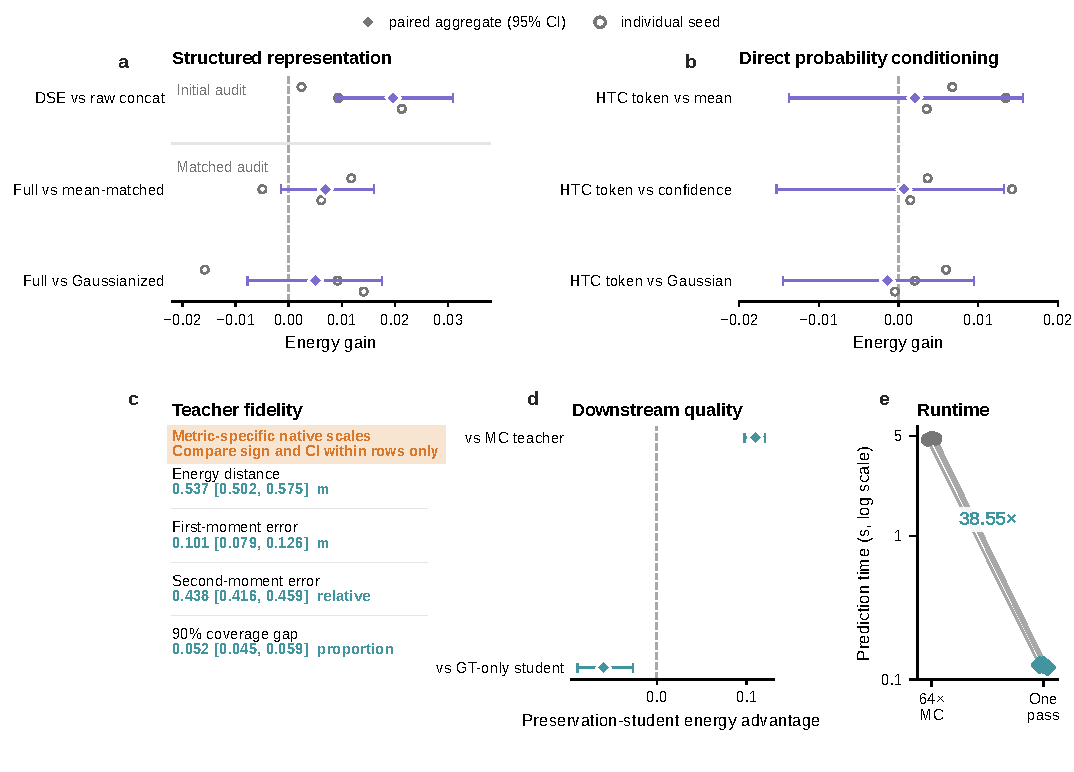
\includegraphics[width=0.96\textwidth]{figure_4_learned_interfaces.pdf}
\caption{Original learned-interface and preservation results. Aggregate effects use paired scene-bootstrap 95\% CIs; open circles show repetitions. Panels (a)--(b) compare encoders and HTC tokens with controls; (c) compares teacher discrepancies within each metric; (d) compares preservation ES with the teacher and GT-only student; and (e) shows three paired timing measurements over 34,856 targets. The 90\% coverage gap in (c) is coverage-status disagreement with the teacher.}
\label{fig:figure4}
\end{figure*}

\subsection{Learned-interface gains varied across populations}
\label{subsec:section5-6}

The direct HTC token improved over mean-only under rotation and temporal offset, but not translation. Final validation favored the token over mean-only by 0.02702 m (0.01588, 0.03932) and over confidence by 0.02092 m (0.01112, 0.03217), with all three repetitions positive. The average structured-encoder and HTC-versus-Gaussian-token contrasts also favored HTC, but included repetition-level reversals (Table 3). HiVT representation and preservation interfaces were not evaluated.

\begin{table*}[!t]
\caption{Original final-validation results. ES effects are baseline minus candidate; area ratios are candidate/baseline at empirical 90\% coverage. Effects average three paired repetitions with scene-bootstrap 95\% CIs; signs give individual directions.}
\label{tab:table3}
\centering
\footnotesize
\setlength{\tabcolsep}{3pt}
\renewcommand{\arraystretch}{1.15}
\begin{tabularx}{\textwidth}{@{}>{\hsize=0.8\hsize\linewidth=\hsize}Y>{\hsize=1.1\hsize\linewidth=\hsize}Y>{\hsize=1.0\hsize\linewidth=\hsize}Y>{\hsize=1.6\hsize\linewidth=\hsize}Y>{\hsize=0.85\hsize\linewidth=\hsize}Y>{\hsize=0.65\hsize\linewidth=\hsize}Y@{}}
\toprule
\textbf{Level} & \textbf{Candidate} & \textbf{Baseline} & \textbf{Trajectory ES effect, m (95\% CI)} & \textbf{Area ratio \(\downarrow\)} & \textbf{Repetition signs} \\
\midrule
Stochastic, CV & HTC & Gaussian & 0.02060 (0.01632, 0.02532) & 0.8549 & + / + / + \\
Stochastic, MLP & HTC & Gaussian & 0.02101 (0.01603, 0.02688) & 0.8537 & + / + / + \\
\addlinespace[1pt]
Structured representation & Full HTC encoder & Mean-matched & 0.03115 (0.01784, 0.04570) & 1.0728 & + / + / - \\
Structured representation & Full HTC encoder & Gaussianized encoder & 0.02827 (0.01518, 0.04142) & 0.9648 & + / + / - \\
\addlinespace[1pt]
Direct conditioning & HTC token & Mean-only & 0.02702 (0.01588, 0.03932) & 0.9874 & + / + / + \\
Direct conditioning & HTC token & Confidence & 0.02092 (0.01112, 0.03217) & 0.9849 & + / + / + \\
Direct conditioning & HTC token & Gaussian token & 0.01682 (0.00456, 0.03051) & 0.9723 & + / - / + \\
\addlinespace[1pt]
Objective & Preservation student & MC teacher & 0.09834 (0.08768, 0.10803) & 0.9427 & + / + / + \\
Objective & Preservation student & GT-only student & -0.01740 (-0.04238, 0.00968) & 2.7151 & - / - / - \\
\bottomrule
\end{tabularx}
\end{table*}

\begin{figure*}[!t]
\centering
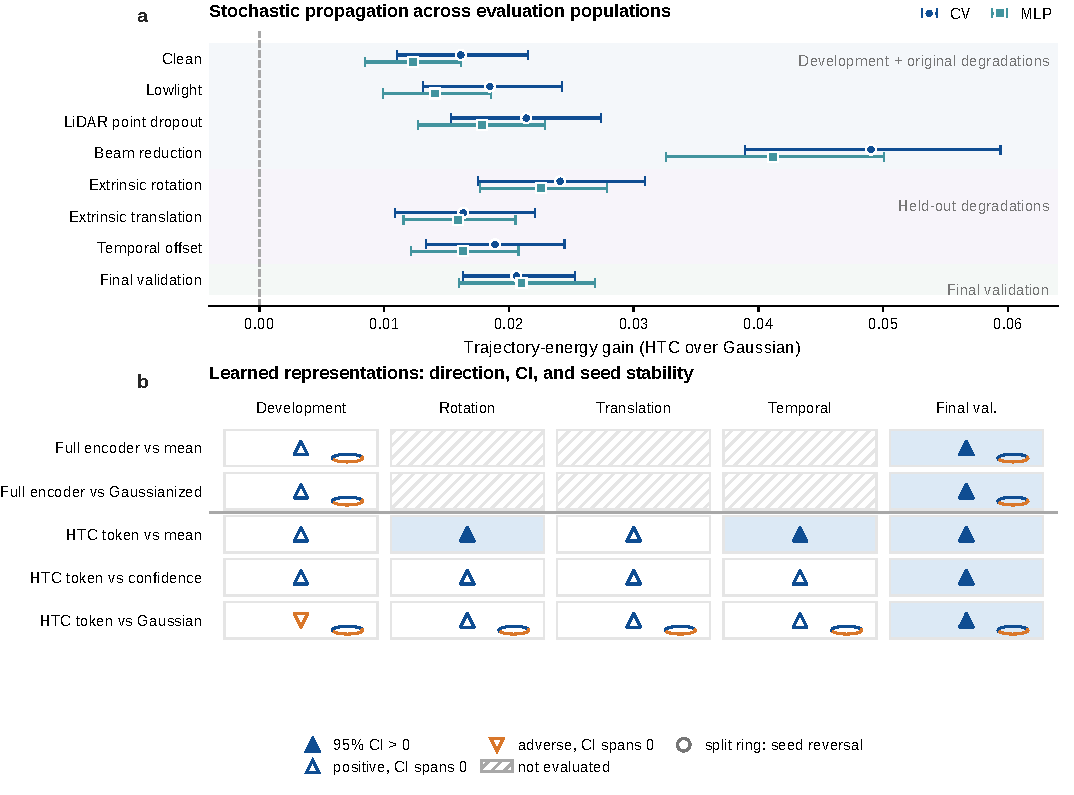
\includegraphics[width=0.98\textwidth]{figure_5_interface_stability.pdf}
\caption{Original-study results across evaluation populations. Panel (a) gives G-minus-HTC ES for CV/MLP with scene-bootstrap 95\% CIs. Panel (b) summarizes learned-interface effects: filled upward triangles, CI above zero; open upward triangles, positive estimate with CI spanning zero; downward triangles, negative estimate with CI spanning zero; hatching, unevaluated; split rings, repetition reversals.}
\label{fig:figure5}
\end{figure*}

\subsection{Forecast-error ranking captured complementary utility}
\label{subsec:section5-7}

Original final-validation HTC-over-G high-FDE AUPRC gains were 0.03099 (0.02033, 0.04185) for CV and 0.01988 (0.01034, 0.02946) for MLP. The direct token improved risk--coverage over mean-only and confidence on development and final validation, but did not outperform the Gaussian token on final-validation ranking endpoints (Supplementary Fig. S3). These results identify a use of probability inputs for prioritizing large forecast errors alongside scoring the full predictive law.

\section{Discussion}
\label{sec:section6}

\subsection{Law value depends on the host and comparator}
\label{subsec:section6-1}

The original CV/MLP experiments consistently favored HTC over both the trained Gaussian law and its moment-matched surrogate. HiVT preserved the moment-matched advantage while leaving the trained-law comparison unresolved. G and HTC-MMG answer different questions: G is an independently trained predictive law, whereas HTC-MMG replaces HTC's shape at fixed input moments. The positive surrogate contrast therefore supports value beyond the current XY mean and covariance in HiVT, without establishing superiority over the trained Gaussian.

The extension changes input coordinates, context, and native future law together. Its evidence therefore concerns the complete forecasting configuration and motivates evaluating uncertainty in the intended host.

\subsection{Representation utility and teacher fidelity address different goals}
\label{subsec:section6-2}

Future-supervised predictors already observe history and mean state, while confidence and Gaussian scale can carry information correlated with HTC parameters. This may help explain why learned-interface gains depend on the comparator and population. Final-validation tokens improved over mean-only and confidence consistently across repetitions, even though development ES gains were unresolved.

Preservation training made the student more faithful to its teacher, but did not establish better forecasting than matched GT-only training. The tested loss recipe rewards teacher properties that need not optimize accuracy against future labels.

\section{Conclusion}
\label{sec:section7}

Perception uncertainty has distinct propagation, representation, and training-objective uses. HTC improved stochastic forecasting in CV/MLP across six degradation families. In HiVT, HTC improved over a moment-matched Gaussian but was not clearly separated from the trained Gaussian law. Learned conditioning showed comparator- and population-dependent benefits, while preservation improved teacher fidelity without establishing a GT-only forecasting advantage. These findings support evaluating each interface in its intended host configuration with a control matched to the question.

\section*{Data Availability}

This study uses nuScenes under its license. Derived target metadata, degradation definitions, and result archives are retained with integrity metadata. The release package is being prepared in the \url{https://github.com/JayceZhou/multimodal-uq}; an archival identifier and redistribution policy remain to be finalized.

\section*{Code Availability}

The code repository for this study is \url{https://github.com/JayceZhou/multimodal-uq}.

\section*{Author Contributions}

{\small \textbf{Shencheng Zhou:} Conceptualization, Methodology, Software, Investigation, Data curation, Formal analysis, Validation, Visualization, Writing -- original draft. \textbf{Xinyuan Zhang:} Formal analysis, Validation, Writing -- review \& editing. \textbf{Quan Qian:} Conceptualization, Resources, Supervision, Project administration, Funding acquisition, Writing -- review \& editing.\par}

\section*{Competing Interests}

The authors declare no competing interests.

\section*{Acknowledgments}

This work was supported by the Advanced Materials-National Science and Technology Major Project (2025ZD0620100) and the Open Research Fund of Yunnan Tin \& Indium Laboratory (202405AR340002-25EA02).

\begin{thebibliography}{00}

\bibitem{ref1} J. Gao, C. Sun, H. Zhao, \textit{et al.}, ``VectorNet: Encoding HD maps and agent dynamics from vectorized representation,'' in \textit{Proc. IEEE/CVF Conf. Computer Vision and Pattern Recognition (CVPR)}, 2020, pp. 11525--11533. \href{https://openaccess.thecvf.com/content_CVPR_2020/html/Gao_VectorNet_Encoding_HD_Maps_and_Agent_Dynamics_From_Vectorized_Representation_CVPR_2020_paper.html}{Online}

\bibitem{ref2} M. Liang, B. Yang, R. Hu, \textit{et al.}, ``Learning lane graph representations for motion forecasting,'' in \textit{Proc. European Conf. Computer Vision (ECCV)}, 2020. \href{https://www.ecva.net/papers/eccv_2020/papers_ECCV/html/3622_ECCV_2020_paper.php}{Online}

\bibitem{ref3} S. Shi, L. Jiang, D. Dai, and B. Schiele, ``Motion Transformer with global intention localization and local movement refinement,'' in \textit{Advances in Neural Information Processing Systems}, vol. 35, 2022. \href{https://proceedings.neurips.cc/paper_files/paper/2022/hash/2ab47c960bfee4f86dfc362f26ad066a-Abstract-Conference.html}{Online}

\bibitem{ref4} A. Seff, B. Cera, D. Chen, \textit{et al.}, ``MotionLM: Multi-agent motion forecasting as language modeling,'' in \textit{Proc. IEEE/CVF Int. Conf. Computer Vision (ICCV)}, 2023, pp. 8579--8590. \href{https://openaccess.thecvf.com/content/ICCV2023/html/Seff_MotionLM_Multi-Agent_Motion_Forecasting_as_Language_Modeling_ICCV_2023_paper.html}{Online}

\bibitem{ref5} Z. Liu, H. Tang, A. Amini, \textit{et al.}, ``BEVFusion: Multi-task multi-sensor fusion with unified bird's-eye view representation,'' in \textit{Proc. IEEE Int. Conf. Robotics and Automation (ICRA)}, 2023, pp. 2774--2781. \href{https://doi.org/10.1109/ICRA48891.2023.10160968}{Online}

\bibitem{ref6} Y. Dong, C. Kang, J. Zhang, \textit{et al.}, ``Benchmarking robustness of 3D object detection to common corruptions,'' in \textit{Proc. IEEE/CVF Conf. Computer Vision and Pattern Recognition (CVPR)}, 2023, pp. 1022--1032. \href{https://openaccess.thecvf.com/content/CVPR2023/html/Dong_Benchmarking_Robustness_of_3D_Object_Detection_to_Common_Corruptions_CVPR_2023_paper.html}{Online}

\bibitem{ref7} L. Kong, Y. Liu, X. Li, \textit{et al.}, ``Robo3D: Towards robust and reliable 3D perception against corruptions,'' in \textit{Proc. IEEE/CVF Int. Conf. Computer Vision (ICCV)}, 2023, pp. 19994--20006. \href{https://openaccess.thecvf.com/content/ICCV2023/html/Kong_Robo3D_Towards_Robust_and_Reliable_3D_Perception_against_Corruptions_ICCV_2023_paper.html}{Online}

\bibitem{ref8} G. P. Meyer, A. Laddha, E. Kee, C. Vallespi-Gonzalez, and C. K. Wellington, ``LaserNet: An efficient probabilistic 3D object detector for autonomous driving,'' in \textit{Proc. IEEE/CVF Conf. Computer Vision and Pattern Recognition (CVPR)}, 2019, pp. 12677--12686. \href{https://openaccess.thecvf.com/content_CVPR_2019/html/Meyer_LaserNet_An_Efficient_Probabilistic_3D_Object_Detector_for_Autonomous_Driving_CVPR_2019_paper.html}{Online}

\bibitem{ref9} D. Feng, L. Rosenbaum, C. Glaeser, F. Timm, and K. Dietmayer, ``Can we trust you? On calibration of a probabilistic object detector for autonomous driving,'' arXiv:1909.12358, 2019. \href{https://arxiv.org/abs/1909.12358}{Online}

\bibitem{ref10} X. Gu, G. Song, I. Gilitschenski, M. Pavone, and B. Ivanovic, ``Producing and leveraging online map uncertainty in trajectory prediction,'' in \textit{Proc. IEEE/CVF Conf. Computer Vision and Pattern Recognition (CVPR)}, 2024, pp. 14521--14530. \href{https://openaccess.thecvf.com/content/CVPR2024/html/Gu_Producing_and_Leveraging_Online_Map_Uncertainty_in_Trajectory_Prediction_CVPR_2024_paper.html}{Online}

\bibitem{ref11} B. Ivanovic, Y. Lin, S. Shrivastava, P. Chakravarty, and M. Pavone, ``Propagating state uncertainty through trajectory forecasting,'' in \textit{Proc. IEEE Int. Conf. Robotics and Automation (ICRA)}, 2022, pp. 2351--2358. \href{https://doi.org/10.1109/ICRA46639.2022.9811776}{Online}

\bibitem{ref12} M. Cao, C. Wang, W. Zhao, and Z. Zhang, ``PU-TSI: Interactive vehicle trajectory prediction considering perception information uncertainty,'' \textit{IEEE Internet of Things Journal}, vol. 12, no. 15, pp. 30518--30532, 2025. \href{https://doi.org/10.1109/JIOT.2025.3570741}{Online}

\bibitem{ref13} Z. Zhang, X. Qiu, B. Zhang, \textit{et al.}, ``Delving into mapping uncertainty for mapless trajectory prediction,'' in \textit{Proc. IEEE/RSJ Int. Conf. Intelligent Robots and Systems (IROS)}, 2025, pp. 16969--16976. \href{https://arxiv.org/abs/2507.18498}{Online}

\bibitem{ref14} P. Gogoi, F. Janjoš, B. Yang, and A. Look, ``Uncertainty matters: Structured probabilistic online mapping for motion prediction in autonomous driving,'' arXiv:2603.20076, 2026. \href{https://doi.org/10.48550/arXiv.2603.20076}{Online}

\bibitem{ref15} J. Sun, H. Zhang, G. Ding, and Z. Zheng, ``Uncertainty-aware trajectory prediction: A unified framework harnessing positional and semantic uncertainties,'' arXiv:2603.29362, 2026. \href{https://doi.org/10.48550/arXiv.2603.29362}{Online}

\bibitem{ref16} S. Salehi, L. Lusvarghi, M. Sepulcre, and J. Gozalvez, ``Mind the noise: Sensitivity of Transformer-based interaction-aware trajectory prediction models to noisy data,'' in \textit{Proc. IEEE Vehicular Technology Conf. (VTC-Spring)}, Nice, France, 2026. \href{https://doi.org/10.48550/arXiv.2606.21344}{Online}

\bibitem{ref17} H. Wang, J. Hu, W. Wang, and H. Liu, ``Toward trustworthy autonomous driving through the quantification and propagation of uncertainty from HD maps to trajectory prediction,'' \textit{IEEE Transactions on Intelligent Transportation Systems}, early access, Aug. 3, 2026, doi: 10.1109/TITS.2026.3713330. \href{https://doi.org/10.1109/TITS.2026.3713330}{Online}

\bibitem{ref18} M. Liang, B. Yang, W. Zeng, \textit{et al.}, ``PnPNet: End-to-end perception and prediction with tracking in the loop,'' in \textit{Proc. IEEE/CVF Conf. Computer Vision and Pattern Recognition (CVPR)}, 2020, pp. 11553--11562. \href{https://openaccess.thecvf.com/content_CVPR_2020/html/Liang_PnPNet_End-to-End_Perception_and_Prediction_With_Tracking_in_the_Loop_CVPR_2020_paper.html}{Online}

\bibitem{ref19} A. Hu, Z. Murez, N. Mohan, \textit{et al.}, ``FIERY: Future instance prediction in bird's-eye view from surround monocular cameras,'' in \textit{Proc. IEEE/CVF Int. Conf. Computer Vision (ICCV)}, 2021, pp. 15273--15282. \href{https://openaccess.thecvf.com/content/ICCV2021/html/Hu_FIERY_Future_Instance_Prediction_in_Birds-Eye_View_From_Surround_Monocular_ICCV_2021_paper.html}{Online}

\bibitem{ref20} Y. Zhang, Z. Zhu, W. Zheng, \textit{et al.}, ``BEVerse: Unified perception and prediction in bird's-eye-view for vision-centric autonomous driving,'' arXiv:2205.09743, 2022. \href{https://arxiv.org/abs/2205.09743}{Online}

\bibitem{ref21} J. Gu, C. Hu, T. Zhang, \textit{et al.}, ``ViP3D: End-to-end visual trajectory prediction via 3D agent queries,'' in \textit{Proc. IEEE/CVF Conf. Computer Vision and Pattern Recognition (CVPR)}, 2023, pp. 5496--5506. \href{https://openaccess.thecvf.com/content/CVPR2023/html/Gu_ViP3D_End-to-End_Visual_Trajectory_Prediction_via_3D_Agent_Queries_CVPR_2023_paper.html}{Online}

\bibitem{ref22} Y. Hu, J. Yang, L. Chen, \textit{et al.}, ``Planning-oriented autonomous driving,'' in \textit{Proc. IEEE/CVF Conf. Computer Vision and Pattern Recognition (CVPR)}, 2023, pp. 17853--17862. \href{https://openaccess.thecvf.com/content/CVPR2023/html/Hu_Planning-Oriented_Autonomous_Driving_CVPR_2023_paper.html}{Online}

\bibitem{ref23} Z. Zhou, L. Ye, J. Wang, K. Wu, and K. Lu, ``HiVT: Hierarchical vector transformer for multi-agent motion prediction,'' in \textit{Proc. IEEE/CVF Conf. Computer Vision and Pattern Recognition (CVPR)}, 2022, pp. 8823--8833. \href{https://openaccess.thecvf.com/content/CVPR2022/html/Zhou_HiVT_Hierarchical_Vector_Transformer_for_Multi-Agent_Motion_Prediction_CVPR_2022_paper.html}{Online}

\bibitem{ref24} K. Wang, C. Shen, X. Li, and J. Lu, ``Uncertainty quantification for safe and reliable autonomous vehicles: A review of methods and applications,'' \textit{IEEE Transactions on Intelligent Transportation Systems}, vol. 26, no. 3, pp. 2880--2896, Mar. 2025, doi: 10.1109/TITS.2025.3532803. \href{https://doi.org/10.1109/TITS.2025.3532803}{Online}

\bibitem{ref25} X. Weng, B. Ivanovic, K. Kitani, and M. Pavone, ``Whose track is it anyway? Improving robustness to tracking errors with affinity-based trajectory prediction,'' in \textit{Proc. IEEE/CVF Conf. Computer Vision and Pattern Recognition (CVPR)}, 2022, pp. 6563--6572. \href{https://openaccess.thecvf.com/content/CVPR2022/html/Weng_Whose_Track_Is_It_Anyway_Improving_Robustness_to_Tracking_Errors_CVPR_2022_paper.html}{Online}

\bibitem{ref26} P. Zhang, L. Bai, Y. Wang, J. Fang, J. Xue, N. Zheng, and W. Ouyang, ``Towards trajectory forecasting from detection,'' \textit{IEEE Transactions on Pattern Analysis and Machine Intelligence}, vol. 45, no. 10, pp. 12550--12561, 2023. \href{https://doi.org/10.1109/TPAMI.2023.3274686}{Online}

\bibitem{ref27} S. Fadadu, S. Pandey, D. Hegde, \textit{et al.}, ``Multi-view fusion of sensor data for improved perception and prediction in autonomous driving,'' in \textit{Proc. IEEE/CVF Winter Conf. Applications of Computer Vision (WACV)}, 2022, pp. 2349--2357. \href{https://openaccess.thecvf.com/content/WACV2022/html/Fadadu_Multi-View_Fusion_of_Sensor_Data_for_Improved_Perception_and_Prediction_WACV_2022_paper.html}{Online}

\bibitem{ref28} S. Papais, L. Wang, B. Cheong, and S. L. Waslander, ``ForeSight: Multi-view streaming joint object detection and trajectory forecasting,'' in \textit{Proc. IEEE/CVF Int. Conf. Computer Vision (ICCV)}, 2025, pp. 25474--25484. \href{https://openaccess.thecvf.com/content/ICCV2025/html/Papais_ForeSight_Multi-View_Streaming_Joint_Object_Detection_and_Trajectory_Forecasting_ICCV_2025_paper.html}{Online}

\bibitem{ref29} A. Malinin, B. Mlodozeniec, and M. Gales, ``Ensemble distribution distillation,'' in \textit{Proc. 8th Int. Conf. Learning Representations (ICLR)}, 2020. \href{https://openreview.net/forum?id=BygSP6Vtvr}{Online}

\bibitem{ref30} L. Ding, D. Li, B. Liu, \textit{et al.}, ``Safe motion planning for autonomous vehicles by quantifying uncertainties of deep learning-enabled environment perception,'' \textit{IEEE Transactions on Intelligent Vehicles}, vol. 9, no. 1, pp. 2318--2332, 2024. \href{https://doi.org/10.1109/TIV.2023.3297735}{Online}

\bibitem{ref31} N. Grabowsky, A. M\"{u}tze, and M. Rottmann, ``Does knowledge about perceptual uncertainty help an agent in automated driving?'' in \textit{Proc. IEEE/CVF Conf. Computer Vision and Pattern Recognition Workshops (CVPRW)}, 2026, pp. 4219--4229. \href{https://openaccess.thecvf.com/content/CVPR2026W/SAIAD/html/Grabowsky_Does_Knowledge_About_Perceptual_Uncertainty_Help_an_Agent_in_Automated_CVPRW_2026_paper.html}{Online}

\bibitem{ref32} N. Shahroudi, M. Lepson, and M. Kull, ``Evaluation of trajectory distribution predictions with energy score,'' in \textit{Proc. 41st Int. Conf. Machine Learning (ICML)}, PMLR 235, 2024, pp. 44322--44341. \href{https://proceedings.mlr.press/v235/shahroudi24a.html}{Online}

\bibitem{ref33} T. Gneiting and A. E. Raftery, ``Strictly proper scoring rules, prediction, and estimation,'' \textit{Journal of the American Statistical Association}, vol. 102, no. 477, pp. 359--378, 2007. \href{https://doi.org/10.1198/016214506000001437}{Online}

\bibitem{ref34} S. H. Sun, R. Walters, J. Li, and R. Yu, ``Probabilistic symmetry for multi-agent dynamics,'' in \textit{Proc. 5th Annual Learning for Dynamics and Control Conf.}, PMLR 211, 2023, pp. 1231--1244. \href{https://proceedings.mlr.press/v211/sun23a.html}{Online}

\bibitem{ref35} H. Caesar, V. Bankiti, A. H. Lang, \textit{et al.}, ``nuScenes: A multimodal dataset for autonomous driving,'' in \textit{Proc. IEEE/CVF Conf. Computer Vision and Pattern Recognition (CVPR)}, 2020, pp. 11621--11631. \href{https://arxiv.org/abs/1903.11027}{Online}

\end{thebibliography}

% TODO before submission: add the IEEE-compliant AI-use disclosure to Acknowledgments if applicable.
\end{document}
